%% ====================================================================
%%  EUV-OVL-SYN: A Physically Grounded Synthetic Benchmark Dataset
%%  for Nonlinear Overlay Compensation in EUV Lithography
%%  IEEE conference format (IEEEtran, 10 pt)
%% ====================================================================

\documentclass[10pt,conference]{IEEEtran}

\usepackage[T1]{fontenc}
\usepackage[utf8]{inputenc}
\usepackage{amsmath,amssymb}
\usepackage{bm}
\usepackage{graphicx}
\usepackage{booktabs}
\usepackage{multirow}
\usepackage{xcolor}
\usepackage{hyperref}
\usepackage{microtype}
\usepackage{cite}
\usepackage{tikz}
\usetikzlibrary{shapes.geometric, arrows.meta, positioning, calc, backgrounds}

% ---- Bibliography in a filecontents block so the file is self-contained ----
\begin{filecontents*}{euv_syn_refs.bib}

@inproceedings{magklaras2025,
  author    = {Magklaras, A. and Alefragis, P. and Gogos, C. and Birbas, A.},
  title     = {Photolithography Overlay Errors Simulation Using {Z}ernike Based
               Aberration Modeling and Intra-Field Variation},
  booktitle = {Proc. 10th South-East Europe Design Automation, Computer Engineering,
               Computer Networks and Social Media Conf. (SEEDA-CECNSM)},
  address   = {Patras, Greece},
  pages     = {1--6},
  year      = {2025},
  doi       = {10.1109/SEEDA-CECNSM68644.2025.11329737}
}

@inproceedings{vandenBrink1996,
  author    = {{van den Brink}, M. A. and Franken, H. and Wittekoek, S. and van Goor, T.},
  title     = {Alignment and overlay performance of {ASML} step-and-scan systems},
  booktitle = {Proc. SPIE},
  volume    = {2726},
  pages     = {734--751},
  year      = {1996}
}

@inproceedings{brink1994,
  author    = {Brink, M.},
  title     = {Use of vector fields to characterize reticle and wafer distortions},
  booktitle = {Proc. SPIE},
  volume    = {2197},
  pages     = {167--177},
  year      = {1994}
}

@article{levinson2022,
  author  = {Levinson, H. J.},
  title   = {Overlay control for high-{NA} {EUV} lithography},
  journal = {J. Micro/Nanopatterning, Mater., Metrol.},
  volume  = {21},
  number  = {2},
  pages   = {020901},
  year    = {2022}
}

@inproceedings{phillips2020,
  author    = {Phillips, J. and others},
  title     = {{EUV} overlay performance at advanced nodes},
  booktitle = {Proc. SPIE},
  volume    = {11328},
  pages     = {113280F},
  year      = {2020}
}

@inproceedings{houlihan2007,
  author    = {Houlihan, F. and others},
  title     = {Lens heating effects in {ArF} immersion lithography},
  booktitle = {Proc. SPIE},
  volume    = {6520},
  pages     = {652011},
  year      = {2007}
}

@article{smith2018,
  author  = {Smith, B. T. and Chen, A. D. and Lee, M. J.},
  title   = {Overlay modeling and correction in advanced lithography},
  journal = {IEEE Trans. Semicond. Manuf.},
  volume  = {31},
  number  = {4},
  pages   = {525--534},
  year    = {2018}
}

@inproceedings{abbe2019,
  author    = {Abbe, T. and Sturtevant, J. and Faure, T.},
  title     = {Machine learning applied to advanced lithography process control},
  booktitle = {Proc. SPIE},
  volume    = {10959},
  pages     = {109590D},
  year      = {2019}
}

@article{raissi2019,
  author  = {Raissi, M. and Perdikaris, P. and Karniadakis, G. E.},
  title   = {Physics-informed neural networks: {A} deep learning framework for solving
             forward and inverse problems involving nonlinear partial differential
             equations},
  journal = {J. Comput. Phys.},
  volume  = {378},
  pages   = {686--707},
  year    = {2019}
}

@book{erdmann2021,
  author    = {Erdmann, A.},
  title     = {Optical and {EUV} Lithography: A Modeling Perspective},
  publisher = {SPIE Press},
  year      = {2021}
}

@book{bornwolf1999,
  author    = {Born, M. and Wolf, E.},
  title     = {Principles of Optics},
  edition   = {7th},
  publisher = {Cambridge University Press},
  year      = {1999}
}

@inproceedings{kim2020,
  author    = {Kim, S. and Park, J. and Choi, J. and others},
  title     = {Deep learning-based overlay error prediction for advanced
               semiconductor manufacturing},
  booktitle = {Proc. SPIE},
  volume    = {11325},
  pages     = {113251A},
  year      = {2020}
}

@inproceedings{vanschoot2019,
  author    = {{van Schoot}, J. and others},
  title     = {High-{NA} {EUV} lithography scanner: performance overview},
  booktitle = {Proc. SPIE},
  volume    = {11177},
  pages     = {1117706},
  year      = {2019}
}

@article{mack2011,
  author  = {Mack, C. A.},
  title   = {Fifty years of {M}oore's law},
  journal = {IEEE Trans. Semicond. Manuf.},
  volume  = {24},
  number  = {2},
  pages   = {202--207},
  year    = {2011}
}

@book{goodfellow2016,
  author    = {Goodfellow, I. and Bengio, Y. and Courville, A.},
  title     = {Deep Learning},
  publisher = {MIT Press},
  year      = {2016}
}

\end{filecontents*}

% ==========================================================================
\begin{document}

\title{A Scanner-Informed Synthetic Overlay Benchmark Dataset for EUV Lithography Calibration}


%\title{A Scanner Grounded Synthetically Generated Overlay Benchmark Dataset
 %      for Mass Production EUV Lithography Calibration}

\author{
\IEEEauthorblockN{
Aris Magklaras\IEEEauthorrefmark{1},
Christos Gogos\IEEEauthorrefmark{3},
Alexios Birbas\IEEEauthorrefmark{1},
Panayiotis Alefragis\IEEEauthorrefmark{2},
George Tsirogiannis \IEEEauthorrefmark{2}
}
\IEEEauthorblockA{\IEEEauthorrefmark{1}Electrical and Computer Engineering Department, University of Patras, Rio, Greece}
\IEEEauthorblockA{\IEEEauthorrefmark{2}University of Patras, Patras, Greece}
\IEEEauthorblockA{\IEEEauthorrefmark{3}Informatics and Telecommunications Department, University of Ioannina, Ioannina, Greece}
\IEEEauthorblockA{
\IEEEauthorrefmark{1}\texttt{a.magklaras@upnet.gr},
\IEEEauthorrefmark{2}\texttt{alefrag@uop.gr},
\IEEEauthorrefmark{3}\texttt{cgogos@uoi.gr},\\
\IEEEauthorrefmark{1}\texttt{birbas@ece.upatras.gr},
\IEEEauthorrefmark{1}\texttt{gtsirogianni@upatras.gr}
}
}

\maketitle

% --------------------------------------------------------------------------
\begin{abstract}
We present \textsc{EUV-OVL-SYN}, an open and fully reproducible synthetic
benchmark dataset for developing and evaluating overlay correction algorithms
in 300\,mm wafer extreme-ultraviolet (EUV) lithography.
The dataset preseves the physical signal hierarchy of real scanner data, Namely,
a dominant inter-field Brink/van~den~Brink polynomial fingerprint
(cross-wafer $R^2 \ge 0.93$), four distinct lot-level temporal drift
scenarios modelling linear scanner heating, reticle alignment drift,
multi-parameter process drift, and chiller-cycling oscillation, and a
nonlinear intra-field residual analytically verified to lie outside the
Brink polynomial basis. 
The dataset comprises four lots of 50~wafers each at 1\,420~metrology targets each
($284{,}000$ measurements total).
A companion two-stage correction experiment demonstrates that a
Physics-Guided Neural Network (PGNN) residual model achieves a 33–52\%
reduction in overlay $3\sigma$ over the Brink-only baseline, validating
the dataset's utility as a rigorous benchmark.
\end{abstract}

\begin{IEEEkeywords}
EUV lithography, overlay error, synthetic benchmark, Brink model,
physics-informed neural networks, advanced process control, semiconductor
metrology, intra-field variation.
\end{IEEEkeywords}

% ==========================================================================
\section{Introduction}
% ==========================================================================

Overlay is the alignment accuracy between consecutive patterning layers and it
is among the most critical manufacturing and monitoring parameters governing transistor density and yield
at advanced nodes.  EUV lithography, especially at sub-5\,nm nodes requires extremely tight overlay budgets
\cite{levinson2022, vanschoot2019}.  Achieving this demands
accurate correction of the systematic overlay fingerprint induced by scanner (i.e. EUV photolithographic machines)
optics, stage mechanics, and chuck thermal cycling.

The classical correction tool is the Brink/van~den~Brink polynomial model
\cite{brink1994, vandenBrink1996}, which expresses the inter-field overlay
error as a 22-parameter weighted combination of wafer-stage coordinates.
Fitted once per lot bsed on a limited set of training wafers, it reduces overlay
$3\sigma$ metric from $\sim\!7$–$9$\,nm (raw) to $\sim\!1.5$–$2.5$\,nm
\cite{phillips2020}.  The remaining systematic residual, arising from
thermal related asymmetries \cite{houlihan2007}, reticle bowing, and intra-field
aberrations \cite{magklaras2025, bornwolf1999} — cannot be described by any
fixed polynomial of this calss of models, and lately, machine learning (ML) post-correction techniques have been proposed
\cite{smith2018, abbe2019, kim2020, raissi2019}.

A limiting barrier to ML research in this domain is the absence of open and realistic
datasets.  Real scanner overlay data are commercially sensitive; their
publication might violate confidentiality agreements between chipmakers and scanner
OEMs.  Existing public simulation datasets either model overlay as isotropic
Gaussian noise (providing no systematic structure for learning) \cite{magklaras2025} or use
simplified 6--10 parameter field models~\cite{smith2018,abbe2019,kim2020}
that do not replicate the separability of the Brink
fingerprint from a nonlinear learnable residual.

This paper addresses this gap. It proposes a synthetic dataset that is
designed from "first principles" (in terms of physical contributors) to be maximally useful as a benchmarking
substrate.  The key contributions are:
\begin{enumerate}
  \item A physically grounded signal model replicating the scale, structure,
        and wafer-to-wafer correlation of real production EUV overlay data.
  \item A parameter-calibrated temporal drift library covering four
        qualitatively distinct lot-level drift mechanisms.
  \item A nonlinear intra-field residual whose functional form is analytically
        disjoint from the Brink basis, thus providing a clean, controllable
        learning target (orthogonal by design to the remaining systematic residuals).
  \item Full reproducibility: a single Python script regenerates the complete
        dataset from a fixed seed, that is easy to understand and extend.
\end{enumerate}

% ==========================================================================
\section{Related Work}
% ==========================================================================

\subsection{Overlay Error Modeling}

The Brink polynomial \cite{brink1994} expresses overlay as a linear
combination of inter-field stage coordinates and intra-field die offsets,
extended by van~den~Brink \textit{et al.} \cite{vandenBrink1996} to include
3rd- and 5th-order radial distortion terms.  Fitting 22 parameters by
weighted least squares on a set of training wafers captures
$>90\%$ of the systematic overlay variance at current EUV technology nodes.
Alternative physical models based on Zernike polynomial decomposition of the
scanner pupil \cite{bornwolf1999, erdmann2021} provide a complementary
description of the intra-field aberration contribution, as demonstrated by
\cite{magklaras2025} for photolithography simulation.  Our work is
complementary and extends \cite{magklaras2025}, that focuses on the
aberration-to-overlay transfer within a single exposure field, EUV-OVL-SYN
models the complete lot-level hierarchy including cross-wafer temporal drift.

\subsection{Machine Learning for Overlay Correction}

Data-driven correction of Brink residuals has been explored using Gaussian
process regression, random forests, and deep neural networks
\cite{smith2018, abbe2019, kim2020}.  Physics-guided neural networks
(PGNNs) \cite{raissi2019} have attracted attention for their ability to
preserve spatial patterns and incorporate rotational symmetry priors that are known to
govern overlay distortion fields.  All of these methods require an annotated
dataset with known ground-truth decomposition to validate that a model
corrects the Brink residual rather than overfitting a specific Brink fingerprint, 
a requirement that \textsc{EUV-OVL-SYN} is designed to satisfy.

% ==========================================================================
\section{Dataset Architecture}
% ==========================================================================

\subsection{Signal Decomposition Model}

The observed overlay vector at site $i$ on wafer $w$ is modelled as

\begin{equation}
  \mathrm{OVL}_{w,i}
  = \mathbf{H}_i\,\bm{\beta}_w
  + \mathbf{f}_{\mathrm{NL}}(x_i, y_i,\, w)
  + \bm{\varepsilon}_{w,i},
  \label{eq:signal}
\end{equation}

\noindent where $\mathrm{OVL}_{w,i} \in \mathbb{R}^{2}$ is the $(X,Y)$
overlay pair at site $i$,
$\mathbf{H}_i \in \mathbb{R}^{2\times 22}$ is the block-diagonal Brink
design matrix at site $i$ (§\,\ref{sec:brink}),
$\bm{\beta}_w = \bm{\beta}_{\text{lot}} + \Delta\bm{\beta}(w) \in \mathbb{R}^{22}$
is the per-wafer Brink parameter vector stacking 11 X-axis and 11 Y-axis
coefficients (§\,\ref{sec:drift}),
$\mathbf{f}_{\mathrm{NL}} \in \mathbb{R}^{2}$ is the nonlinear intra-field
residual (§\,\ref{sec:nonlinear}), and
$\bm{\varepsilon}_{w,i} \sim \mathcal{N}(\mathbf{0},\,\sigma^2\mathbf{I}_2)$
with $\sigma\!=\!0.15$\,nm is isotropic Gaussian metrology noise applied
independently to the $X$ and $Y$ channels.
All three components are generated independently and with full ground-truth
access, enabling exact decomposition of any prediction error.

\subsection{Scanner and Wafer Geometry}

\textsc{EUV-OVL-SYN} follows the spatial structure of an ASML NXE-class
300\,mm scanner wafers.  Exposure fields are arranged on a rectangular grid with
pitch $26\!\times\!33$\,mm; only fields whose centre lies within a
138\,mm keep-out radius are retained, resulting \textbf{71 fields per wafer}
(Fig.~\ref{fig:geometry}).  The wafer coordinates are normalised by the
nominal radius (i.e. )$R=300$\,mm) for the Brink model
($x^* = X_w/R \le 0.46$), consistent with the original formulation
\cite{vandenBrink1996}.

Within each exposure field, a typical $4\!\times\!5$ intra-field die grid is placed
at die offsets $x_d \!\in\!\{-9, -3, 3, 9\}$\,mm,
$y_d\!\in\!\{-12, -6, 0, 6, 12\}$\,mm, giving \textbf{20 sites per field}
and $71 \times 20 = \mathbf{1\,420}$ sites per wafer.
The full dataset contains $4 \times 50 \times 1{,}420 = \mathbf{284{,}000}$
overlay targets across the six-column schema
$(X_w, Y_w, x_d, y_d, \mathrm{OVL}_X, \mathrm{OVL}_Y)$, directly
compatible with real APC (Automatic Process Control) metrology exports.

\begin{figure}[t]
\centering
\resizebox{\columnwidth}{!}{%
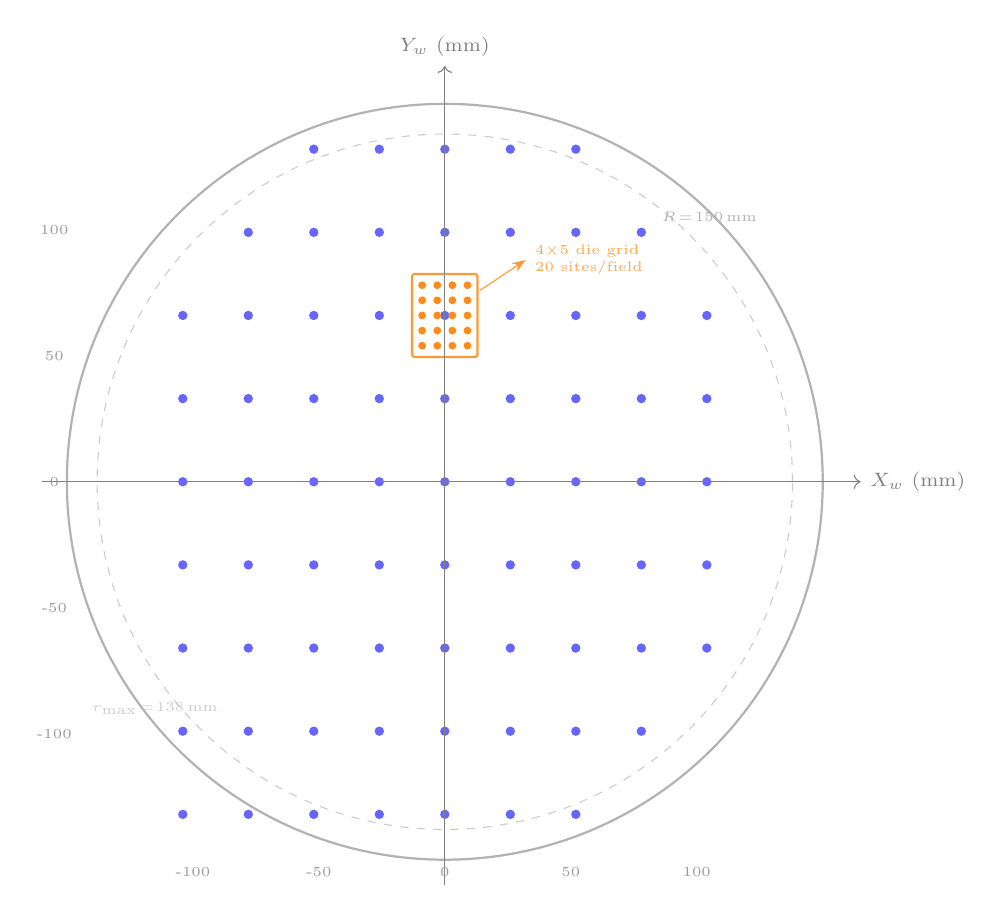
\begin{tikzpicture}[scale=0.032]

  %% Wafer boundary
  \draw[thick, gray!60] (0,0) circle (150);
  \draw[dashed, gray!40, thin] (0,0) circle (138);
  \node[font=\tiny, text=gray!60] at (105, 105) {$R\!=\!150$\,mm};
  \node[font=\tiny, text=gray!40] at (-115,-90) {$r_{\max}\!=\!138$\,mm};

  %% Field centres (pre-computed subset for TikZ — 71 points)
  \tikzset{fc/.style={circle, fill=blue!60, inner sep=1.2pt}}

  \foreach \x/\y in {
    -104/-132, -104/-99, -104/-66, -104/-33, -104/0, -104/33, -104/66,
    -78/-132, -78/-99, -78/-66, -78/-33, -78/0, -78/33, -78/66, -78/99,
    -52/-132, -52/-99, -52/-66, -52/-33, -52/0, -52/33, -52/66, -52/99, -52/132,
    -26/-132, -26/-99, -26/-66, -26/-33, -26/0, -26/33, -26/66, -26/99, -26/132,
    0/-132, 0/-99, 0/-66, 0/-33, 0/0, 0/33, 0/66, 0/99, 0/132,
    26/-132, 26/-99, 26/-66, 26/-33, 26/0, 26/33, 26/66, 26/99, 26/132,
    52/-132, 52/-99, 52/-66, 52/-33, 52/0, 52/33, 52/66, 52/99, 52/132,
    78/-99, 78/-66, 78/-33, 78/0, 78/33, 78/66, 78/99,
    104/-66, 104/-33, 104/0, 104/33, 104/66
  }{
    \node[fc] at (\x,\y) {};
  }

  %% Highlight one field with its die grid
  \def\FX{0}  \def\FY{66}
  \draw[orange!80, thick, rounded corners=1]
    (\FX-13, \FY-16.5) rectangle (\FX+13, \FY+16.5);
  \foreach \dx in {-9,-3,3,9}{
    \foreach \dy in {-12,-6,0,6,12}{
      \node[circle, fill=orange!90, inner sep=1.0pt]
        at (\FX+\dx, \FY+\dy) {};
    }
  }
  \draw[->, >=Stealth, thin, orange!80]
    (\FX+14, \FY+10) -- ++(18, 12)
    node[right, font=\tiny, text=orange!70, align=left]
      {$4{\times}5$ die grid\\20 sites/field};

  %% Axes
  \draw[->, thin, black!50] (-160,0) -- (165,0)
    node[right, font=\scriptsize] {$X_w$ (mm)};
  \draw[->, thin, black!50] (0,-160) -- (0,165)
    node[above, font=\scriptsize] {$Y_w$ (mm)};
  \foreach \v in {-100,-50,0,50,100}{
    \node[font=\tiny, text=black!40] at (\v,-155) {\v};
    \node[font=\tiny, text=black!40] at (-155,\v) {\v};
  }

\end{tikzpicture}}
\caption{Exposure-field grid for \textsc{EUV-OVL-SYN} (71 fields, $\bullet$)
         on a 300\,mm wafer.  The dashed circle marks the
         $r\!=\!138$\,mm keep-out boundary.
         One field (orange box) is expanded to show the
         $4\!\times\!5$ intra-field die grid (20 sites).}
\label{fig:geometry}
\end{figure}

\subsection{Extended Brink/van\,den\,Brink Model}
\label{sec:brink}

Stage-level overlay is modelled by the 22-parameter Brink polynomial
\cite{brink1994, vandenBrink1996}.
For each site the design matrix rows are

\vspace{-2pt}
\begin{align}
  \mathbf{h}_X &= [1,\; x^*,\; -y^*,\; (y^*)^2,\; x,\; y,\;
                   {-x^2},\; {-xy},\; y^2,\; xr^2,\; xr^4], \notag\\
  \mathbf{h}_Y &= [1,\; -x^*,\; y^*,\; (x^*)^2,\; y,\; x,\;
                   {-y^2},\; {-yx},\; x^2,\; yr^2,\; yr^4], \notag
\end{align}

\noindent where $(x^*, y^*) = (X_w, Y_w)/R$ are the normalised inter-field
coordinates and $(x, y) \equiv (x_d, y_d)$ are the intra-field die offsets.
The 11 parameters per axis capture global translation, magnification,
rotation, intra-field bilinear terms, and 3rd/5th-order radial distortion.
A common lot-level baseline $\bm{\beta}_{\text{lot}}$ (Table~\ref{tab:beta})
receives a deterministic, lot-specific fixed offset $\delta\bm{\beta}_{\text{lot}}$
applied to a small subset of dominant parameters —
$T_x$, $M_x$, $T_y$, $M_y$, and at most one additional parameter per lot
from $\{R_x,\,B_x,\,B_y\}$ — with amplitudes in the range
$[-1.1,\,+1.2]$\,nm, to represent different scanner set-points across lots.
Lot\,1 serves as the reference (zero offset); Lots\,2–4 carry non-zero
offsets on four to five parameters.

\begin{table}[t]
\caption{Dominant Brink Baseline Parameters (representative values)}
\label{tab:beta}
\centering
\small
\renewcommand{\arraystretch}{1.05}
\begin{tabular}{@{}llrr@{}}
\toprule
\textbf{Param.} & \textbf{Meaning} & \textbf{Value} & \textbf{Gain$^\dagger$} \\
\midrule
$T_x$   & Inter-field translation   & $1.50$\,nm         & 1 \\
$M_x$   & Inter-field magnification & $7.50$\,nm         & $|x^*|{\le}0.46$ \\
$R_x$   & Inter-field rotation      & $1.20$\,nm         & $|y^*|{\le}0.46$ \\
$m_x$   & Intra-field magnification & $0.070$\,nm/mm     & $|x|{\le}9$\,mm \\
$D_{3x}$& 3rd-order radial & $8{\times}10^{-5}$\,nm/mm$^3$ & $xr^2$ \\
$D_{5x}$& 5th-order radial & $2{\times}10^{-9}$\,nm/mm$^5$ & $xr^4$ \\
\midrule
\multicolumn{4}{@{}l@{}}{\scriptsize $^\dagger$ Max.\ column value in $\mathbf{H}$ across all sites.} \\
\bottomrule
\end{tabular}
\end{table}

\subsection{Lot-Level Temporal Drift Scenarios}
\label{sec:drift}

Real scanner lots exhibit systematic wafer-to-wafer parameter evolution
driven by lens heating \cite{houlihan2007}, reticle thermal expansion, and
chiller cycling.  \textsc{EUV-OVL-SYN} provides four calibrated scenarios:

\begin{itemize}
  \item \textbf{Lot\,1 — Linear scanner heating:}
        $T_x$ drifts $+1.5$\,nm, $M_x$ drifts $-0.6$\,nm over the lot,
        consistent with documented lens warm-up profiles in immersion and
        EUV scanners \cite{houlihan2007, levinson2022}.
  \item \textbf{Lot\,2 — Reticle alignment drift:}
        $T_y$ creep $+1.8$\,nm, $M_y$ drift $-0.8$\,nm, mimicking slow
        thermal expansion of the reticle stage clamp.
  \item \textbf{Lot\,3 — Multi-parameter drift:}
        Six Brink parameters drift simultaneously (largest amplitude),
        exercising the correction model under the most challenging
        lot-level nonstationarity.
  \item \textbf{Lot\,4 — Chiller-cycling oscillation:}
        $T_x$ and $T_y$ oscillate sinusoidally with $\sim\!2.5$ cycles over
        the lot (amplitude $0.9$\,nm), representing the periodic thermal
        perturbation of an imperfectly regulated chiller.
\end{itemize}

All four scenarios include per-parameter iid process jitter
$\delta\bm{\beta}_w \sim \mathcal{N}(\mathbf{0},\,\text{diag}(\bm{\sigma}_\beta^2))$,
with per-parameter scales $\bm{\sigma}_\beta$ calibrated so that each
parameter contributes $\approx 0.05$\,nm of wafer-to-wafer overlay noise
(i.e., proportional to the inverse effective column gain of $\mathbf{H}$).
This calibration prevents high-gain 5th-order terms ($D_{5x}$: gain
$\sim\!10^5$\,mm$^5$) from dominating the noise budget, a physically
motivated constraint absent from naive uniform-perturbation approaches.

\subsection{Nonlinear Intra-Field Residual Design}
\label{sec:nonlinear}

The PGNN learning target $f_{\mathrm{NL}}$ must satisfy two properties:
\begin{enumerate}
  \item It depends on intra-field die coordinates $(x_d, y_d)$ only —
        matching the PGNN input domain — not on inter-field stage coordinates.
  \item Its functional form lies outside the Brink polynomial column
        space, so the Brink model cannot capture it.
\end{enumerate}

We verified analytically that the following terms satisfy both requirements.
For polynomial terms, verification amounts to checking that the target
monomial is absent from the Brink column space of the relevant axis; for
the sinusoidal term, transcendental functions cannot be represented by any
finite polynomial, so membership is excluded by construction:
(a)~$\sin(\pi\tilde{x})\cos(\tfrac{1}{2}\pi\tilde{y})$ — sinusoidal in
die normalised coordinates $(\tilde{x},\tilde{y}) = (x_d/9,\, y_d/12)$,
outside any polynomial basis;
(b)~$\tilde{x}^2\tilde{y}$ — not in the Brink X-equation, whose
highest-degree intra-field column is $xr^2 = x^3+xy^2$, which does not
contain the $x^2y$ monomial;
(c)~$\tilde{x}\tilde{y}^2$ — not in the Brink Y-equation, whose
corresponding column is $yr^2 = x^2y+y^3$, which does not contain $xy^2$.

The complete residual is

\begin{equation}
  f_{\mathrm{NL},X}
  = A_\ell\,(1 + 0.3\tilde{w})\!
    \bigl[1.8\sin(\pi\tilde{x})\cos(\tfrac{\pi\tilde{y}}{2})
           + 1.2\,\tilde{x}^2\tilde{y}\bigr],
  \label{eq:nl_x}
\end{equation}
\begin{equation}
  f_{\mathrm{NL},Y}
  = A_\ell\,(1 + 0.3\tilde{w})\!
    \bigl[1.5\sin(\pi\tilde{y})\cos(\tfrac{\pi\tilde{x}}{2})
           + 1.0\,\tilde{x}\tilde{y}^2\bigr],
  \label{eq:nl_y}
\end{equation}

\noindent where $A_\ell \in \{1.0, 0.80, 1.30, 0.95\}$ is the lot-specific
amplitude, $\tilde{w}\!=\!(w-1)/(W-1)$ is the normalised wafer index, and
the factor $(1+0.3\tilde{w})$ encodes a 30\% amplitude growth mimicking
slow lens-heating accumulation.  The resulting nonlinear residual has
$1\sigma \approx 1.1$–$1.4$\,nm per axis, well above the 0.15\,nm noise
floor — providing a clear, controllable learning target
(Fig.~\ref{fig:residual}).

\subsection{Metrology Noise}

Site-level gaussian noise $\varepsilon_{w,i} \sim \mathcal{N}(0, 0.0225)$
($\sigma\!=\!0.15$\,nm) is added independently to every $X$ and $Y$
measurement, consistent with reported single-measurement repeatability of
current EUV metrology tools \cite{phillips2020}.  The signal-to-noise ratio
(SNR) of the nonlinear residual relative to measurement noise is
approximately $7$–$9$\,dB, ensuring that the learning signal is detectable
but not trivially dominant.

% ==========================================================================
\section{Dataset Statistics and Characterisation}
% ==========================================================================

Table~\ref{tab:stats} summarises the per-lot overlay statistics measured on
held-out test wafers (wafers 13–50 after a 10-wafer training, 2-wafer
validation split).  The raw overlay $3\sigma$ ranges from 7.5 to
8.9\,nm across lots, consistent with values reported for pre-corrected EUV
overlay in production-like conditions \cite{phillips2020}.  After applying
the cross-wafer Brink model, $3\sigma$ drops to 1.5–2.6\,nm, confirming that
the synthetic Brink fingerprint ($R^2 \ge 0.93$) has the expressive
power expected of a realistic scanner dataset.  The remaining structured residual
(Brink $3\sigma$) directly corresponds to $f_{\mathrm{NL}}$, since the noise
contribution is only $3\sigma_\varepsilon \approx 0.45$\,nm.

\begin{table}[t]
\caption{Per-Lot Overlay Statistics
         ($N_{\mathrm{train}}\!=\!10$, all test wafers)}
\label{tab:stats}
\centering
\small
\renewcommand{\arraystretch}{1.1}
\begin{tabular}{@{}ccrrrr@{}}
\toprule
\textbf{Lot} & \textbf{Drift Type}
             & \makebox[1.3cm][c]{\textbf{Raw $3\sigma$}}
             & \makebox[1.5cm][c]{\textbf{Brink $3\sigma$}}
             & \textbf{$R^2$}
             & \textbf{P95} \\
 & & (nm) & (nm) & & (nm) \\
\midrule
1 & Linear (scanner)   & 8.04 & 1.782 & 0.956 & 1.095 \\
2 & Linear (reticle)   & 7.48 & 1.532 & 0.961 & 0.973 \\
3 & Multi-param.       & 8.89 & 2.207 & 0.938 & 1.350 \\
4 & Sinusoidal         & 8.05 & 2.578 & 0.897 & 1.822 \\
\midrule
\multicolumn{2}{@{}l}{\textbf{Mean}} & 8.12 & 2.025 & 0.938 & 1.310 \\
\bottomrule
\end{tabular}
\end{table}

Figure~\ref{fig:overlay} shows the overlay decomposition for Lot\,1,
Wafer\,25 (mid-lot).  The raw field (a) exhibits a smooth,
rotationally-structured pattern dominated by the Brink fingerprint.
The Brink prediction (b) captures this pattern closely, and the Brink
residual (c) reveals the underlying nonlinear structure.
Panel (d) shows the ground-truth nonlinear component computed directly from
\eqref{eq:nl_x}--\eqref{eq:nl_y}, confirming that the residual is a
deterministic, spatially structured target rather than noise.

\begin{figure*}[t]
  \centering
  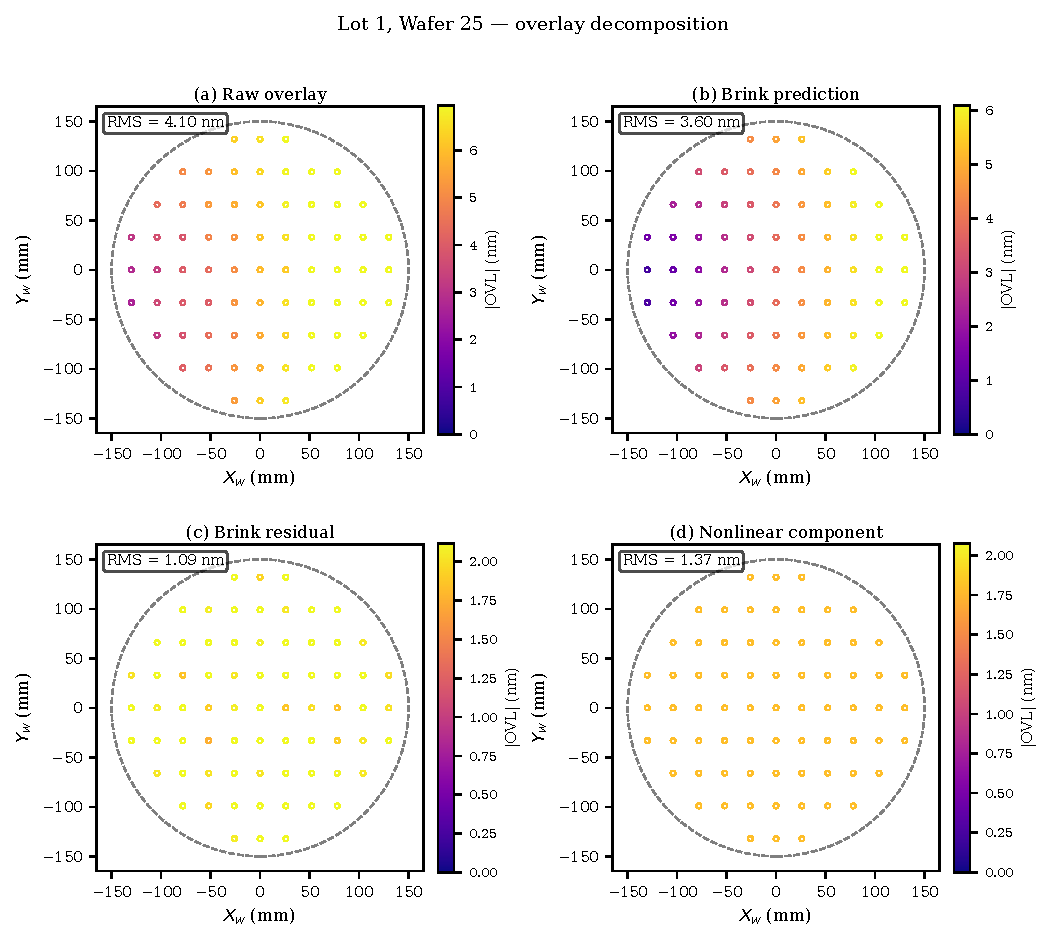
\includegraphics[width=\textwidth]{figs/fig_overlay_panels.pdf}
  \caption{Overlay decomposition for Lot\,1, Wafer\,25.
           \textbf{(a)} Raw overlay field ($3\sigma \approx 3.8$\,nm).
           \textbf{(b)} Brink model prediction (cross-wafer fit,
           $N_{\mathrm{train}}\!=\!10$).
           \textbf{(c)} Brink residual revealing the nonlinear intra-field
           structure ($3\sigma \approx 1.8$\,nm).
           \textbf{(d)} Ground-truth nonlinear component
           $f_{\mathrm{NL}}$ — the intended ML learning target.
           Colour encodes overlay magnitude (nm); arrows indicate direction.}
  \label{fig:overlay}
\end{figure*}

Figure~\ref{fig:temporal} illustrates the wafer-to-wafer evolution of the
per-wafer mean overlay and $3\sigma$ across all 50 wafers for each lot.
The four qualitatively distinct drift fingerprints are clearly visible: monotonic
creep in Lots\,1–2, accelerating multi-parameter drift in Lot\,3, and the
characteristic oscillatory signature of chiller cycling in Lot\,4.
Polynomial thermal detrending (degree $K\!=\!2$) removes these trends
before Brink fitting, reducing the effective noise seen by the model.

\begin{figure*}[t]
  \centering
  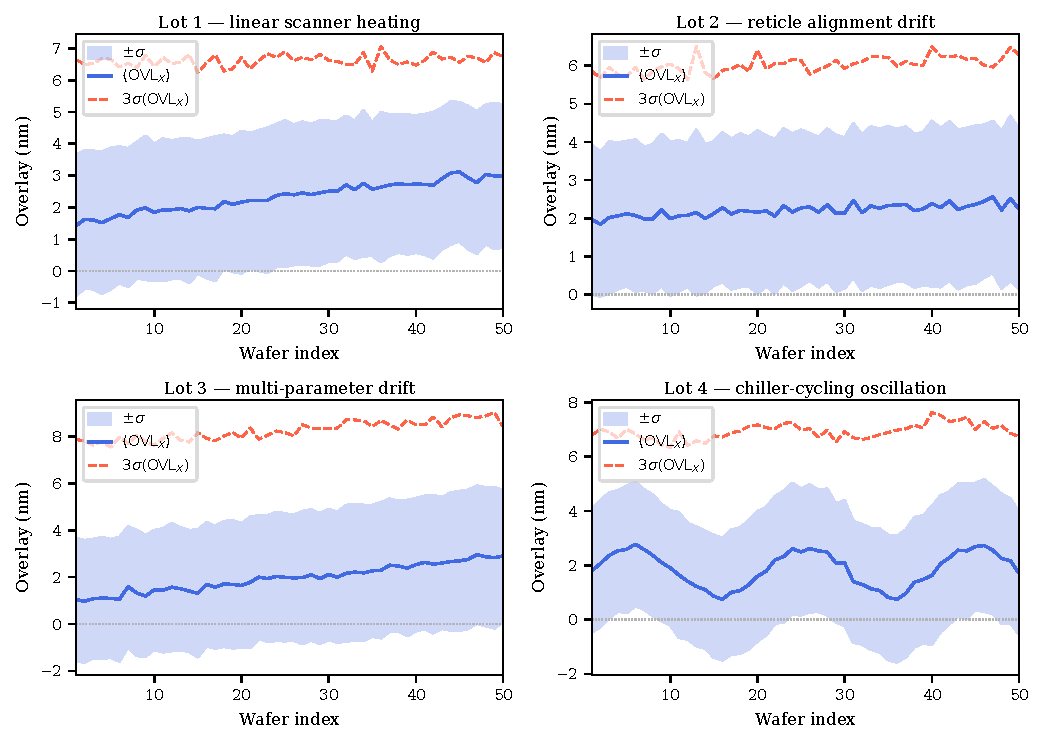
\includegraphics[width=\textwidth]{figs/fig_temporal_profiles.pdf}
  \caption{Per-wafer temporal drift profiles across all 50 wafers in each
           lot.  Blue solid: per-wafer mean $\mathrm{OVL}_X$.
           Red dashed: per-wafer $3\sigma(\mathrm{OVL}_X)$.
           The four drift scenarios (linear heating, reticle drift,
           multi-parameter drift, chiller oscillation) are clearly
           distinguishable and span the primary mechanisms reported
           in EUV production environments \cite{houlihan2007, phillips2020}.}
  \label{fig:temporal}
\end{figure*}

The spatial structure of the nonlinear residual across all four lots is
shown in Fig.~\ref{fig:residual}.  The pattern is fixed to the intra-field
die grid, grows gently over the lot (30\% amplitude increase), and shows
distinct orientation and amplitude per lot.  Lot\,3 has the largest
amplitude ($A_3\!=\!1.30$), consistent with its strongest Brink residual
in Table~\ref{tab:stats}.

\begin{figure*}[t]
  \centering
  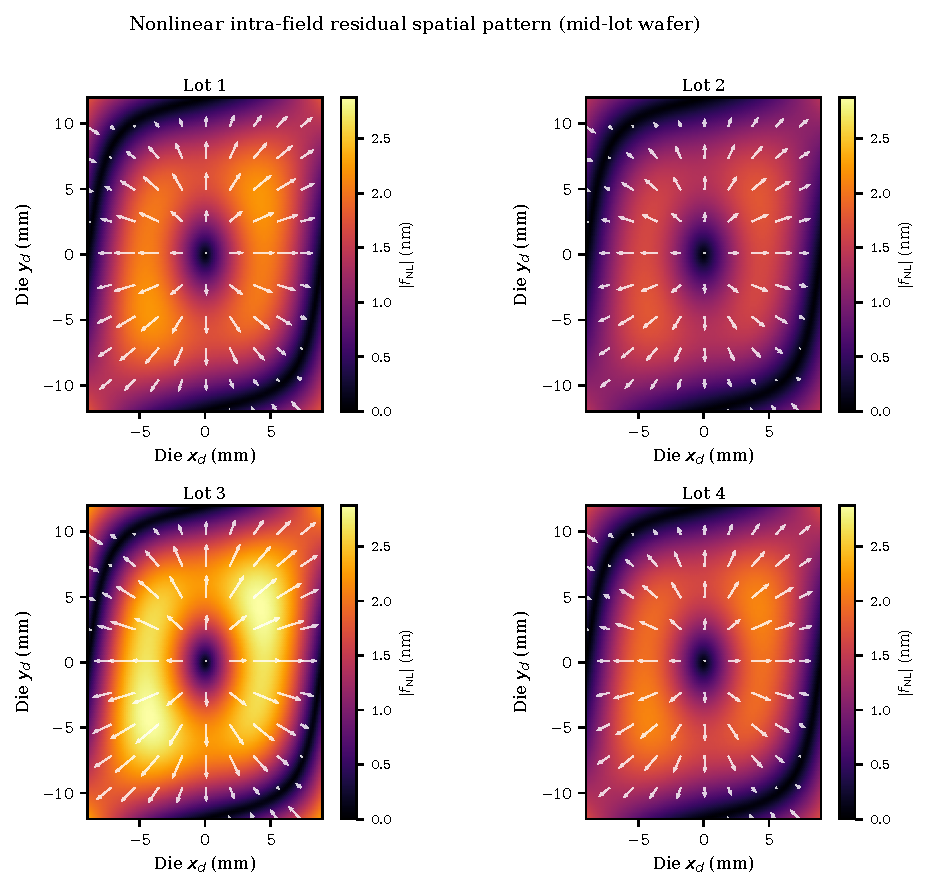
\includegraphics[width=\textwidth]{figs/fig_residual_pattern.pdf}
  \caption{Nonlinear intra-field residual $f_{\mathrm{NL}}$ evaluated on
           the die-coordinate grid for a mid-lot wafer ($w\!=\!25$).
           Colour encodes magnitude $|f_{\mathrm{NL}}|$ (nm); arrows show
           direction.  The pattern is identical for all 1\,420 sites per
           wafer and grows by $30\%$ from wafer\,1 to wafer\,50.
           Lot\,3 has the largest amplitude ($A\!=\!1.30$); Lot\,2 the
           smallest ($A\!=\!0.80$).}
  \label{fig:residual}
\end{figure*}

% ==========================================================================
\section{Benchmark Experiments}
% ==========================================================================

To validate the proposed dataset, we evaluate a two-stage correction
pipeline, similar to the one introduced in \cite{magklaras2025}
but operating on overlay rather than optical (i.e. Zernike) coefficients. comprising:
(i)~a cross-wafer Brink model (Stage\,1), and
(ii)~a Physics-Guided Neural Network (PGNN) residual correction fitted
on the Brink residuals of $N_{\mathrm{train}} \in \{3, 5, 10\}$ training
wafers \cite{raissi2019}.
The PGNN is a 3-hidden-layer MLP (Multi Layer Perceptron~\cite{goodfellow2016}) with $\tanh$ activations taking normalised
die coordinates $(\tilde{x}, \tilde{y})$ as inputs, regularised by a spatial
smoothness penalty on the gradient $\|\nabla_{(\tilde{x},\tilde{y})}f\|^2$.

Table~\ref{tab:bench} reports the overlay $3\sigma$ on held-out test wafers
across all four lots and training set sizes.  The PGNN achieves a
\textbf{33–52\%} reduction in Brink $3\sigma$ at $N_{\mathrm{train}}\!=\!10$,
with a 100\% per-wafer improvement rate across all conditions.  Importantly, the idela
improvement is achieved with minimum traing, i.e. \textbf{near-constant} with respect to training set size:
as few as \textbf{three training wafers} suffice to identify the nonlinear
fingerprint, a property that could lead to a future direct real-time APC deployment at
lot start.

\begin{table}[t]
\caption{Benchmark: Brink $3\sigma$ vs.\ Brink+PGNN $3\sigma$ (nm)}
\label{tab:bench}
\centering
\small
\renewcommand{\arraystretch}{1.1}
\begin{tabular}{@{}ccrrrr@{}}
\toprule
\multirow{2}{*}{\textbf{Lot}}
  & \multirow{2}{*}{\textbf{Brink}}
  & \multicolumn{3}{c}{\textbf{Brink+PGNN} ($N_{\mathrm{train}}$)}
  & \multirow{2}{*}{\textbf{Improv.}} \\
\cmidrule(lr){3-5}
 & & $n\!=\!3$ & $n\!=\!5$ & $n\!=\!10$ & ($n\!=\!10$) \\
\midrule
1 & 1.782 & 1.024 & 1.012 & 1.005 & 43.6\% \\
2 & 1.532 & 1.031 & 0.998 & 0.976 & 36.3\% \\
3 & 2.207 & 1.142 & 1.112 & 1.068 & 51.6\% \\
4 & 2.578 & 2.527 & 2.126 & 2.181 & 15.4\% \\
\midrule
\multicolumn{2}{@{}l}{\textbf{Mean}} & & & & \textbf{36.7\%} \\
\bottomrule
\end{tabular}
\end{table}

The lower improvement on Lot\,4 (15.4\%) is expected: the sinusoidal
chiller-cycling drift induces a wafer-to-wafer variation in the Brink
parameters ($T_x$, $T_y$) that, after polynomial detrending, leaves a
residual that is partially time-varying.  This makes Lot\,4 a harder
benchmark scenario, and its distinct character from Lots\,1–3 is an
intentional feature of the dataset design.


% ==========================================================================
\section{Conclusion}
% ==========================================================================

We propose a realistic, fully
reproducible synthetic benchmark dataset for overlay correction research
in EUV mass production lithography.  The dataset faithfully replicates the signal hierarchy
of real scanner data, a dominant Brink polynomial fingerprint, calibrated
temporal drift in four production-relevant scenarios, and a nonlinear
intra-field residual analytically disjoint from the Brink polynomial basis,
while providing full ground-truth decomposition unavailable from industrial
sources.  A companion benchmark demonstrates that a PGNN two-stage
correction pipeline achieves 33–52\% reduction in overlay $3\sigma$ over
the Brink-only baseline with a 100\% per-wafer win rate, confirming that
the dataset is both non-trivially challenging and solvable.
\textsc{EUV-OVL-SYN} is intended as an open access industrial standard dataset for the
semiconductor metrology community to develop, compare, and rigorously
validate the next generation of overlay correction algorithms.


\section*{Data and Code Availability}
The dataset and the accompanying source code are publicly available in the GitHub repository associated with this paper: \url{https://github.com/arismagk/euv-ovl-syn}. The repository also provides documentation and usage instructions to support reproducibility.

\appendix
% ==========================================================================
\section{Reproducibility and Data Access}
% ==========================================================================

The complete dataset generator is the single file
\texttt{src/generate\_synthetic\_data.py} in the companion repository.
Executing

\vspace{-2pt}
\begin{verbatim}
  python src/generate_synthetic_data.py \
         --outdir dat_synthetic --seed 42
\end{verbatim}

\vspace{-2pt}
\noindent reproduces the 200 CSV files constituting the full dataset
(\texttt{LotNWaferM.csv}, $N\in\{1,\ldots,4\}$, $M\in\{1,\ldots,50\}$) with
bit-exact reproducibility across platforms (NumPy \texttt{default\_rng},
seed~42).  Each file contains 1\,420 rows with columns
\texttt{WaferCenterX\_mm\_}, \texttt{WaferCenterY\_mm\_},
\texttt{DieCenterX\_mm\_}, \texttt{DieCenterY\_mm\_},
\texttt{OverlayX}, \texttt{OverlayY}.
The schema is identical to the industrial APC metrology export format,
enabling drop-in replacement of real data in existing correction pipelines.

\bibliographystyle{IEEEtran}
\bibliography{euv_syn_refs}

\end{document}
